\documentclass[border=10pt]{standalone}
\usepackage{amsmath}
\usepackage{pgfplots}
\usepgfplotslibrary{fillbetween}
\pgfplotsset{compat=1.18}
\begin{document}
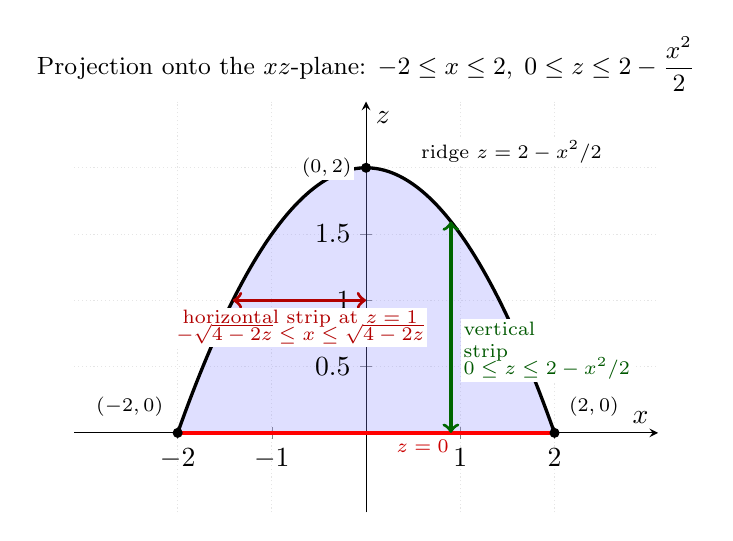
\begin{tikzpicture}
\begin{axis}[width=9cm, height=6.8cm, axis lines=middle,
    xlabel={$x$}, ylabel={$z$}, xmin=-3.1,xmax=3.1, ymin=-0.6,ymax=2.5,
    xtick={-2,-1,1,2}, ytick={0.5,1,1.5,2},
    grid=major, grid style={gray!20,densely dotted}]
  \addplot[name path=RIDGE, blue!45, opacity=0, domain=-2:2, samples=101] {2-x^2/2};
  \addplot[name path=BOT, blue!45, opacity=0, domain=-2:2, samples=2] {0};
  \addplot[fill=blue!45, opacity=0.28] fill between[of=RIDGE and BOT];
  \addplot[very thick, domain=-2:2, samples=101] {2-x^2/2};
  \addplot[red, very thick, domain=-2:2, samples=2] {0};

  \node[font=\scriptsize, align=left, anchor=west, fill=white, inner sep=1pt]
       at (axis cs:0.55,2.12) {ridge $z=2-x^2/2$};
  \node[font=\scriptsize, text=red!80!black, anchor=north, fill=white, inner sep=1pt]
       at (axis cs:0.6,-0.03) {$z=0$};

  \draw[<->, green!40!black, very thick] (0.9,0) -- (0.9,1.595);
  \node[font=\scriptsize, text=green!35!black, align=left, anchor=west, fill=white, inner sep=1pt]
       at (axis cs:1.0,0.62) {vertical\\ strip\\[-2pt] $0\le z\le 2-x^2/2$};

  \draw[<->, red!70!black, very thick] (-1.414,1) -- (0,1);
  \node[font=\scriptsize, text=red!70!black, align=center, anchor=north, fill=white, inner sep=1pt]
       at (axis cs:-0.7,0.95) {horizontal strip at $z=1$\\[-2pt] $-\sqrt{4-2z}\le x\le\sqrt{4-2z}$};

  \addplot[only marks, mark=*, mark size=1.6] coordinates {(-2,0) (2,0) (0,2)};
  \node[font=\scriptsize, anchor=south east] at (axis cs:-2.05,0.05) {$(-2,0)$};
  \node[font=\scriptsize, anchor=south west] at (axis cs:2.05,0.05) {$(2,0)$};
  \node[font=\scriptsize, anchor=east,  fill=white, inner sep=1pt] at (axis cs:-0.12,2.0) {$(0,2)$};
\end{axis}
\node[font=\small, align=center, anchor=south] at (current bounding box.north) {Projection onto the $xz$-plane:  $-2\le x\le 2,\;0\le z\le 2-\dfrac{x^2}{2}$};
\end{tikzpicture}
\end{document}
